\ifx\boi\undefined\ifx\problemname\undefined
\providecommand\sampleinputname{}
\providecommand\sampleoutputname{}
\documentclass[english]{templates/boi}
\problemlanguage{.en}
\fi
\newcommand{\boi}{Baltic Olympiad in Informatics}
\newcommand{\practicesession}{Practice Session}
\newcommand{\contestdates}{April 27 - May 1, 2018}
\newcommand{\dayone}{Day 1}
\newcommand{\daytwo}{Day 2}
\newcommand{\licensingtext}{This problem is licensed under CC BY-SA 4.0.}
\newcommand{\problem}{Problem}
\newcommand{\inputsection}{Input}
\newcommand{\outputsection}{Output}
\newcommand{\interactivity}{Interactivity}
\newcommand{\grading}{Grading}
\newcommand{\scoring}{Scoring}
\newcommand{\constraints}{Constraints}
\renewcommand{\sampleinputname}{Sample Input}
\renewcommand{\sampleoutputname}{Sample Output}
\newcommand{\sampleexplanation}[1]{Explanation of Sample #1}
\newcommand{\sampleexplanations}{Explanation of Samples}
\newcommand{\timelimit}{Time Limit}
\newcommand{\memorylimit}{Memory Limit}
\newcommand{\seconds}{s}
\newcommand{\megabytes}{MB}
\newcommand{\group}{Group}
\newcommand{\points}{Points}
\newcommand{\limitsname}{Limits}
\newcommand{\additionalconstraints}{Additional Constraints}
\newcommand{\testgroups}{
Your solution will be tested on a set of test groups, each worth a number of points.
Each test group contains a set of test cases.
To get the points for a test group you need to solve all test cases in the test group.
Your final score will be the maximum score of a single submission.
}
\fi
\def\version{jury-1}
\problemname{Polygondrama}
Som vi alla vet kan TV-serier med många personer innebära komplicerade kärleksdraman. 
I en TV-serie finns det $N$ personer. Varje person älskar exakt en person, 
vilket faktiskt kan vara den själv.
Två personer är i en relation om och endast om de båda älskar varandra. 


En specifik typ av komplicerat kärleksdrama kallas för ``polygondrama''.
Vi säger att $3$ eller fler personer är i ett ``polygondrama'' om den första personen älskar den andra, 
den andra älskar den tredje, och så vidare, samt att den sista personen älskar den första personen.

Undersökningar har visat att tittarna har blivit trötta på komplicerade kärleksdraman
och skulle föredra något mer romantiskt. Därför bestämmdes det att vissa personer ska 
skjutas med kärlekspilar så att alla hamnar i en relation.
Genom att skjuta en person med en kärlekspil kan du välja att ändra vem den personen 
älskar till vem du vill.

Vad är det minsta antalet kärlekspilar som behövs för att alla ska hamna i en relation?

\section*{\inputsection}
Den första raden innehåller ett heltal $N$, antalet personer.
Nästkommande $N$ rader innehåller två mellanslagsseparerade namn $s$ och $t$, vilket betyder att
personen med namn $s$ älskar personen med namn $t$. Namnen av personerna kommer inte att innehålla
fler än $10$ bokstäver, och alla bokstäver kommer vara små och ingå i det engelska alfabetet.

\section*{\outputsection}
Skriv ut ett heltal -- det minsta antalet kärlekspilar som krävs för att alla ska vara i en
relation. Om det inte är möjligt, skriv ut $-1$.

\section*{\constraints}
\testgroups

\noindent
\begin{tabular}{| l | l | l | l |}
\hline
\group & \points & \limitsname & \additionalconstraints \\ \hline
1     & 21     & $2 \le N \le 20$ & \\ \hline
2     & 25     & $2 \le N \le 100\,000$ & Alla personer är älskade av någon. (Möjligen dem själva) \\ \hline
3     & 29     & $2 \le N \le 100\,000$ & Det finns inga relationer och inga ``polygondraman''. \\ \hline
4     & 25     & $2 \le N \le 100\,000$ & \\ \hline
\end{tabular}

\section*{\sampleexplanations}

\begin{center}
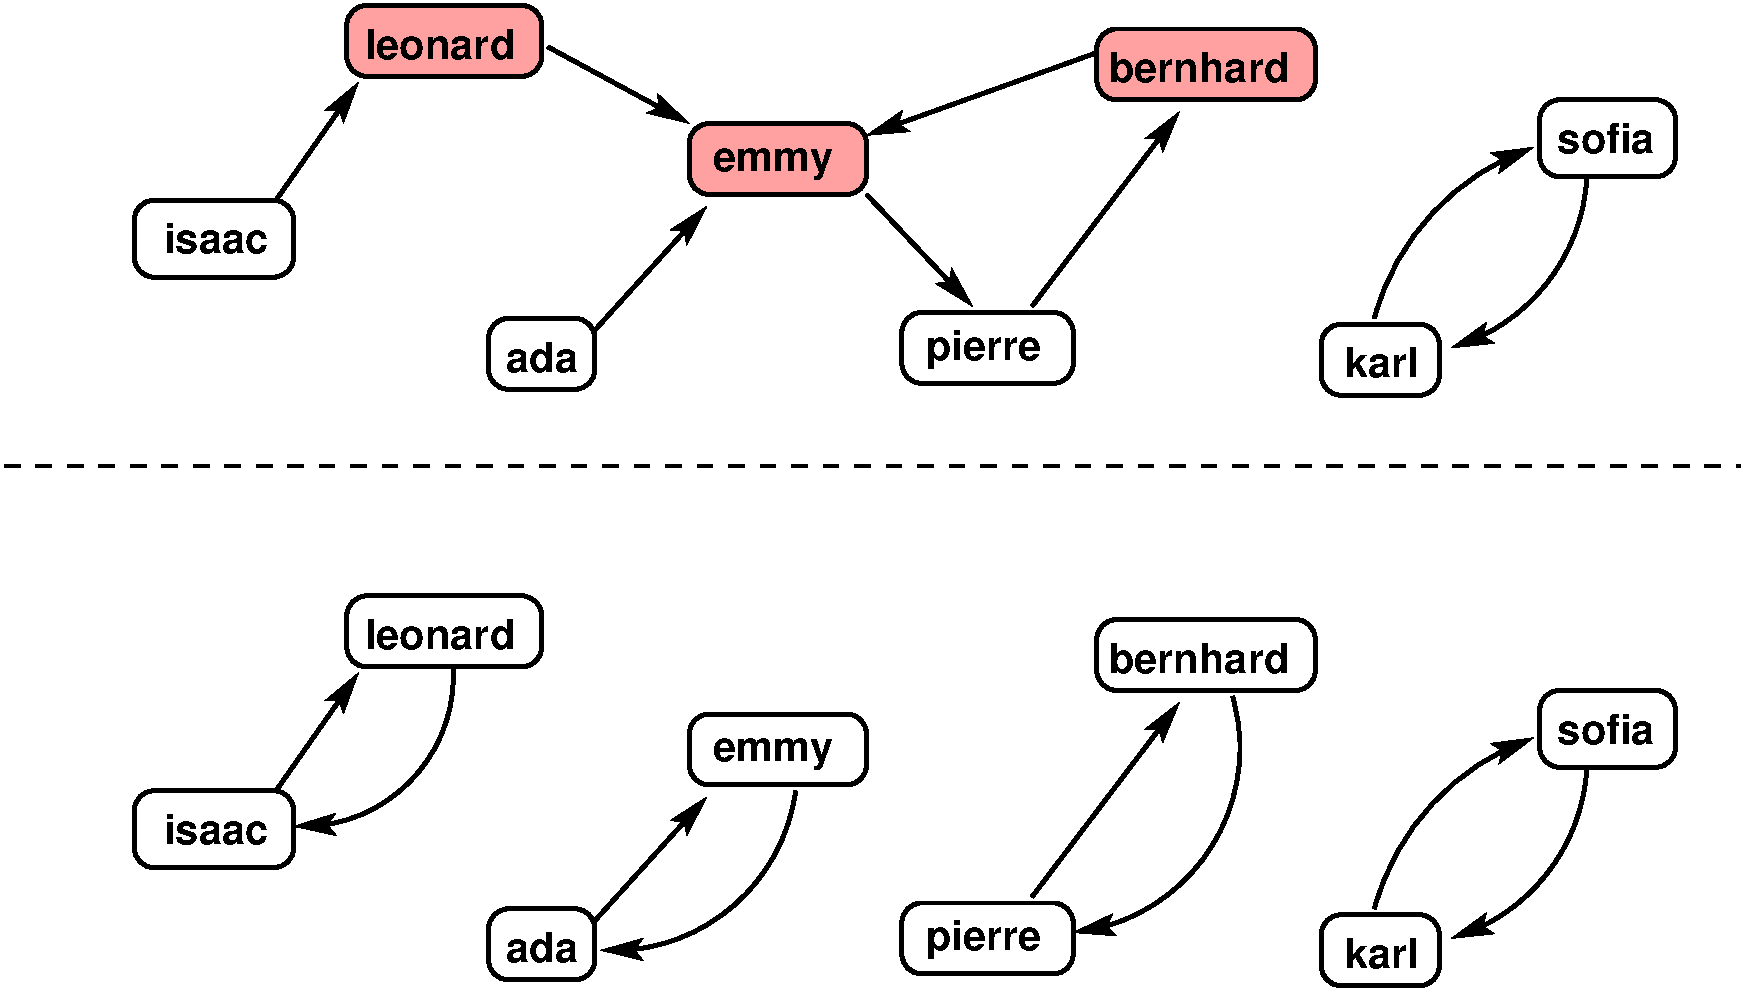
\includegraphics[width=0.5\textwidth]{polygonfig.pdf}
\end{center}
Det första exemplet illustreras i figuren ovan. Den övre delen visar vem som älksar varandra från början, där en pil från $s$ till $t$ indikerar att $s$ älskar $t$,
och den rosa förtydligar de tre personerna som behöver skjutas med en kärlekspil i den unika optimala lösningen. Den undre delen visar situationen efter att kärlekspilarna har skjutits.

I det andra exemplet (där det räcker att skjuta 3 kärlekspilar) finns det flera optimala lösningar.
En av dessa är att skjuta \texttt{a}, \texttt{b} and \texttt{d} med kärlekspilar, och låta dem älska \texttt{b}, \texttt{a} and \texttt{c}, respektive.

I det tredje exemplet har vi ett ``polygondrama'', och oavsätt hur många kärlekspilar som 
skjuts kommer någon inte hamna i en relation.
